\documentclass[letterpaper]{article}
\usepackage[utf8]{inputenc}
\usepackage[spanish]{babel}
\usepackage{amssymb, amsmath}
\usepackage{graphicx}
\usepackage{lipsum}
\usepackage{dsfont}
\usepackage[margin=1.5cm,
vmargin={1cm,0.3cm},
includefoot]{geometry}
\usepackage{setspace}
\usepackage{subcaption}
\usepackage{tocloft}
\usepackage{upgreek}
\usepackage{amsthm}
\usepackage{graphicx}
\usepackage{paralist}
\usepackage{fancyhdr}
\usepackage{lmodern}
\usepackage{tcolorbox}
\usepackage{color}
\usepackage{tikz}
\tcbuselibrary{skins,breakable}
\pagestyle{fancy}

\renewcommand{\headrulewidth}{0.4pt}
\renewcommand{\footrulewidth}{0.4pt}

\providecommand{\abs}[1]{\left|#1\right|}
\providecommand{\norm}[1]{\left|\left|#1\right|\right|}														  
\newcommand{\tq}{ \quad \cdot  \backepsilon \cdot \quad }

\newcommand{\ld}{\lim\limits_{x \to 0^{+}}}

\newcommand{\li}{\lim\limits_{x \to 0^{-}}}

\newcommand{\la}{\lim\limits_{x \to a}}

\newcommand{\R}{\mathds{R}}
\newcommand{\Q}{\mathds{Q}}

\newcommand{\Z}{\mathds{Z}}

\newcommand{\N}{\mathds{N}}

\renewcommand{\P}{\mathcal{P}}

\newcommand{\Po}{\mathds{P}_2(\mathds{R})}

\renewcommand{\*}{\cdot}

\makeatletter
\renewcommand*\env@matrix[1][*\c@MaxMatrixCols c]{%
	\hskip -\arraycolsep
	\let\@ifnextchar\new@ifnextchar
	\array{#1}}
\makeatother

\newtheorem{theorem}{Teorema}[section]
\theoremstyle{definition}
\newtheorem{definition}{Definición}

\begin{document}
\setlength{\unitlength}{1cm}
\thispagestyle{empty}
\begin{picture}(19,3)
\put(-0.5,1.2){
\includegraphics[scale=.20]{unam1.png}}
\put(16,1){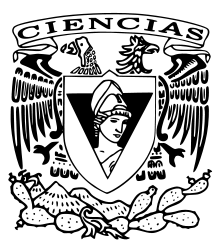
\includegraphics[scale=.29]{fciencias1.png}}
\end{picture}

\begin{center}
	\vspace{-114pt}
	\textbf{\large Álgebra Superior I}\\
	\textbf{ Semestre 2020-2}\\
	Prof. Alejandro Dorantes Aldama\\
	Ayud. Elmer Enrique Tovar Acosta \\
	Ayud. Alejandro Ríos Herrejón \\
	\textbf{Reposición examen I}
\rule{19cm}{0.2mm}
	\vspace{-0.7cm}
	\begin{center}
Kevin Ariel Merino Peña\footnote[2]{Número de cuenta: 317031326}
	\end{center}
	\vspace{-0.5cm}
\rule{19cm}{0.2mm}
\end{center}
 %%%%%%%%%%%%%%%%%%%%%%%%%%%%%%%%%%%%%%%%%%%%
 %			|	EJERCICIO 4					%
 %			|	ARIEL						%	
 %%%%%%%%%%%%%%%%%%%%%%%%%%%%%%%%%%%%%%%%%%%%
\noindent4. Sean A,B conjuntos. Demuestre que las siguientes son equivalentes:
\begin{center}
	1. $ A \subset B \quad$ 2. $ A \cap B = A \quad$ 3. $ A \cup B = B \quad$ 4. $ A \backslash B = \varnothing $
\end{center}
$ 1) \implies 2) $ Supongamos $ A \subseteq B $, por demostrar: $ A \cap B = A $.
\\ $\subseteq]  $
\begin{align*}
	&\text{Supongamos que } & a \in A&\cap B  \\
	&\text{Por definición de intersección } & a \in A &\land a \in  B \\
	&\text{Particularmente } a &\in A \\
	&\text{Entonces } &  A \cap B &\subseteq A 
\end{align*}
$\supseteq]  $
\begin{align*}
	&\text{Supongamos } & a &\in A\\
	&\text{Por hipótesis } & A &\subseteq B \\
	&\text{Particularmente } & a &\in B \\
	&\text{Entonces } & a \in B & \land a \in A\\
	&\text{\textit{i.e.} } & a &\in A \cap B \\
	&\text{Por lo tanto } & A &\subseteq A \cap B 
\end{align*}
\begin{center}
	Como tenemos $ A \subseteq A \cap B  $ y $ A \supseteq A \cap B  $
	$$ \therefore \qquad A = A \cap B  $$
\end{center}
$ 2) \implies 3) $ Supongamos $ A \cap B = A $, por demostrar: $ A \cup B = B $.\\
$\subseteq]  $
\begin{align*}
	& \text{ Supongamos que  } &  a \in& A \cup B \\
	& \text{ Entonces  } &  a \in A &\lor  a \in B
\end{align*}
\begin{align*}
	& \text{\textbf{Caso 1: } Si  } &  a &\in A & \\
	& \text{Entonces } &  a &\in A \cup B \\
	& \text{i.e. } &  a \in A &\land a \in B \\
	& \text{En particular } &  a &\in B\\
	& \text{\textbf{Caso 2}: } a \in B
\end{align*}
Entonces $ A\cup B \subseteq B $\\
$ \supseteq] $
\begin{align*}
	& \text{Supongamos  } &  a &\in B \\
	& \text{Entonces  } &  a &\in A \cup B \\
	& \text{Y así  } &  B &\subseteq A \cup B 
\end{align*}
\begin{center}
	Como $  B \subseteq A \cup B $ y $ A\cup B \subseteq B  $
	\[ \therefore \qquad A\cup B = B \]
\end{center}
$ 3) \implies 4) $ Supongamos $ A \cup B = B $, por demostrar: $ A \backslash B = \varnothing  $.\\
Supongamos $ x \in A \backslash B $, esto es $ a \in A \land a \notin B $, entonces, si $ x \in A \cup B $ y $ A \cup B = B $, entonces
$ x \in B $! lo cual es una contradicción y vino de suponer que hay algún elemento en $ A \backslash B $, por lo que $ A \backslash B = \varnothing $.\\


\noindent$ 4) \implies 1) $ Supongamos $ A \backslash B = \varnothing  $, por demostrar: $ A \subseteq B $.\\
Supongamos que $ a \in A $ y que $ a \notin B $, entonces $ a \in A\backslash B $ pero $ A \backslash B =  \varnothing$! esta contradicción vino de suponer que $ a \notin B $ por lo tanto $ a \in B $ y así $ A \subseteq B $\\


 %%%%%%%%%%%%%%%%%%%%%%%%%%%%%%%%%%%%%%%%%%%%
 %			|	EJERCICIO 8					%
 %			|	ARIEL						%	
 %%%%%%%%%%%%%%%%%%%%%%%%%%%%%%%%%%%%%%%%%%%%
\noindent8. Sean $ A = \{ 1,2,3 \} $ y $ B =\{ 1,2,3,4 \} $. Encuentre todas las parejas ordenadas de $ A \times B $.\\
\[ A \times B = \left\lbrace 
\begin{array}{c}
 (1,1), (1,2), (1,3), (1,4),\\
(2,1), (2,2), (2,3), (2,4),\\
(3,1), (3,2), (3,3), (3,4) 
\end{array}
\right\rbrace \]

 %%%%%%%%%%%%%%%%%%%%%%%%%%%%%%%%%%%%%%%%%%%%
 %			|	EJERCICIO 9					%
 %			|	ARIEL						%	
 %%%%%%%%%%%%%%%%%%%%%%%%%%%%%%%%%%%%%%%%%%%%
\noindent9. Sean $ A = \{ 1,2, \dots, n \} $ y $ B = \{ 1,2, \dots, m \} $. Demuestre que el producto $ A \times B $ tiene $ nm $ elementos. Sugerencia: ¿Cuántas parejas tienen como primera coordenada 1?, ¿y 2?\\

Para cada elemento en $ A $, existirán tantas parejas como elementos de $ B $ \textit{i.e.} si $ A $ tiene $ 3 $ elementos y $ B $ tiene sólo uno entonces las parejas lucirán de la sigueinte forma 
\[ (a,n), (b,n), (c,n) \]
Se podrán combinar tantas veces como elementos haya en $ B $, por lo tanto la cardinalidad de $ A \times B $ es $ nm $ pues por cada elemento en $ A $ se podrán formar tantas parejas como elementos haya en $ B $, puede representarse como:
\[ \text{Elementos de B} \]
\[\text{Elementos de A} \begin{pmatrix}
(x_0,y_0) & (x_0,y_1 ) & \dots m\\
\vdots & \ddots& \vdots\\
n & \dots& nm\\
\end{pmatrix}
\]

 %%%%%%%%%%%%%%%%%%%%%%%%%%%%%%%%%%%%%%%%%%%%
 %			|	EJERCICIO 16				%
 %			|	ARIEL						%	
 %%%%%%%%%%%%%%%%%%%%%%%%%%%%%%%%%%%%%%%%%%%%
\noindent16. Encuentre la imagen de las siguientes funciones:
\[ f : \N \to \N  \text{ dada por } f(n) = n + 1  \]
\[  Img(f) = \N\backslash\{ 1 \}\]
$ \subseteq] $
\begin{align*}
	&\text{Supongamos }	& f(a) &\in Img(f) \\
	&\text{Entonces }	& a &\in \N \\
	&\text{i.e. }	& a &\geq 1 \\
	&\text{Luego, por la regla de correspondencia de  }f	& f(a) &= a + 1 \\
	&\text{Entonces  }	& f(a) &\geq 2\\
	&\text{Así  }	& f(a) &\in  \N\backslash\{ 1 \}\\
	&\text{Por lo que  }	& Img(f) &\subseteq  \N\backslash\{ 1 \}
\end{align*}
$ \supseteq] $
\begin{align*}
	&\text{Supongamos }	& x &\in \N\backslash\{ 1 \} \\
	&\text{Sea }	& a &= x - 1 \\
	&\text{Entonces }	& f(a) &= (x - 1) + 1 \\
	&\text{Así,  }	& f(a) &= x\\
	&\text{Por lo que  }	& \N\backslash\{ 1 \} &\subseteq Img(f)
\end{align*}
\begin{center}
	$ \therefore \N\backslash\{ 1 \} = Img(f) $
\end{center}
\[ f : \N \to \N \text{ dada por } f(n) = n^2 + 1  \]
\[  Img(f) = \N\backslash\{ 1 \}\]
$ \subseteq] $
\begin{align*}
&\text{Supongamos }	& f(a) &\in Img(f) \\
&\text{Entonces }	& a &\in \N \\
&\text{i.e. }	& a &\geq 1 \\
&\text{También veamos que }	& a^2 &\geq 1 \implies a^2 + 1 \geq 1 + 1  \\
&\text{Luego, por la regla de correspondencia de  }f	& f(a) &= a^2 + 1 \\
&\text{Entonces  }	& f(a) &\geq 2\\
&\text{Así  }	& f(a) &\in  \N\backslash\{ 1 \}\\
&\text{Por lo que  }	& Img(f) &\subseteq  \N\backslash\{ 1 \}
\end{align*}
$ \supseteq] $
\begin{align*}
&\text{Supongamos }	& x &\in \N\backslash\{ 1 \} \\
&\text{Sea }	& a &= \sqrt{x - 1} \\
&\text{Entonces }	& f(a) &= (\sqrt{x - 1})^2 + 1 \\
&\text{Así,  }	& f(a) &= x\\
&\text{Por lo que  }	& \N\backslash\{ 1 \} &\subseteq Img(f)
\end{align*}
\begin{center}
	$ \therefore \N\backslash\{ 1 \} = Img(f) $
\end{center}
\[ f : \Z \to \N \text{ dada por } f(n) = n^2 + 1  \]
\[  Img(f) = \N \]
$ \subseteq] $
\begin{align*}
&\text{Supongamos }	& f(a) &\in Img(f) \\
&\text{Entonces }	& a &\in \Z \\
&\text{También veamos que }	& a^2 &\geq 0 \implies a^2 + 1 \geq 1   \\
&\text{Luego, por la regla de correspondencia de  }f	& f(a) &= a^2 + 1 \\
&\text{Entonces  }	& f(a) &\geq 1\\
&\text{Así  }	& f(a) &\in  \N\\
&\text{Por lo que  }	& Img(f) &\subseteq  \N
\end{align*}
$ \supseteq] $
\begin{align*}
&\text{Supongamos }	& x &\in \N \\
&\text{Sea }	& a &= \pm \sqrt{x - 1} \\
&\text{Entonces }	& f(a) &= (\pm \sqrt{x - 1})^2 + 1 \\
&\text{Así,  }	& f(a) &= x\\
&\text{Por lo que  }	& \N &\subseteq Img(f)
\end{align*}
\begin{center}
	$ \therefore \N= Img(f) $
\end{center}
 %%%%%%%%%%%%%%%%%%%%%%%%%%%%%%%%%%%%%%%%%%%%
 %			|	EJERCICIO 17				%
 %			|	ARIEL						%	
 %%%%%%%%%%%%%%%%%%%%%%%%%%%%%%%%%%%%%%%%%%%%
\noindent17. Sean $ f, g: \R \to \R $ dadas por $ f(x) = x + 1 $ y $ g(x) = x^2 $. Calcule $ f \circ g $ y $ g \circ f $.\\

\noindent a) $ f \circ g $
\begin{align*}
	(f \circ g)(x) &= f(g(x)) \qquad \forall x \in \R\\
	& = (x^2) + 1\\
	& = x^2 + 1
\end{align*}
b) $ g \circ f $
\begin{align*}
	(g \circ f)(x) &= g(f(x)) \qquad \forall x \in \R\\
	& = (x+ 1)^2\\
	& = x^2 + 2x + 1
\end{align*}

 %%%%%%%%%%%%%%%%%%%%%%%%%%%%%%%%%%%%%%%%%%%%
 %			|	EJERCICIO 21				%
 %			|	ARIEL						%	
 %%%%%%%%%%%%%%%%%%%%%%%%%%%%%%%%%%%%%%%%%%%%
\noindent21. Como siempre, los símbolos $ \Z $ y $ \Q $ denotarán al conjunto de número enteros y al conjunto de números racionales, respectivamente, ¿Es cierto que 
\[ R:= \left\lbrace \left(\dfrac{m}{n}, \dfrac{1}{n}\right): m, n \in \Z \right\rbrace \]
es una función de $ \Q $ en $ \Q $?\\
Para probar que una realación binaria es una función, debe satisfacer los siguientes enunciados
\begin{itemize}
	\item $ D_R = \Q $
	\item Si $ (x_0, y_1) \in R $ y $ (x_0, y_2) \in R $, entonces $ y_1 = y_2 $
\end{itemize}
Primer requerimiento: \\
$ \subseteq] $ \\
Supongamos $ x \in D_R $ por demostrar $ x \in \Q $
\begin{align*}
	& \text{Como } & x &\in D_R\\
	& \text{Tiene la forma } & x &= \dfrac{m}{n}, \quad m, n \in \Z\\
	& \text{Así como los elementos de  }\Q & x&\in \Q\\
	& \text{Por lo que  } & D_R &\subseteq \Q
\end{align*}
$ \supseteq] $
\begin{align*}
	& \text{Supongamos } & x &\in \Q\\
	& \text{Entonces tiene la siguiente forma } & x &= \dfrac{m}{n}, \quad n, m \in \Z \\
	& \text{Al igual que } D_R & x &\in D_R\\
	& \text{Por lo que  } &  D_R &\supseteq \Q
\end{align*}
\begin{center}
	Como tenemos $ D_R \supseteq \Q  $ y $ D_R \subseteq \Q  $
	\[ \therefore \qquad D_R = \Q  \]
	Y así hemos visto que cumple con la primera condición
\end{center}
Para la segunda condición, tomemos $ \left( \dfrac{1}{2}, \dfrac{1}{2} \right) \in R $ y $ \left( \dfrac{2}{4}, \dfrac{1}{4} \right) \in R $
observemos que $ \dfrac{1}{2} = \dfrac{2}{4} $, pero $ \dfrac{1}{2} \neq \dfrac{1}{4}  $
\begin{center}
	$ \therefore \quad R $ no es función
\end{center}
\end{document}